\chapter{Research Plan}
\label{chap:ResearchPlan}
The main research problem of this dissertation is to determine if we can track automatically and reliably what visual objects, and implicitly what data, users are looking at when interacting with complex, interactive data visualizations (\underline{Contribution-1}); and to find effective ways in which we can interpret and analyze that behavioral data (\underline{Contribution-2}).

\section{Contribution-1: Investigate the feasibility of collecting DOI data in a reliable way.}
\label{sec:Contrib1}

Many eye-tracking related studies generate visual stimuli using computer programs coded by visualization researchers. In such cases, since the structure and layout of the visual content in the stimuli is accessible at runtime, we can relate gaze positions supplied on the fly by an eye-tracker to the visual content of such visualizations.

For example, a network diagram depicting the characters from the novel Les Miserable is shown in Figure~\ref{fig:Miserables}. Links between two characters are present if they co-occurred in the same chapter. The colors indicate different clusters of characters. The visualization has interactions such as dragging nodes (i.e. rectangles). Moreover, users can input a `compactness' value to change the layout of the visualization. The lower value of compactness indicates a dense layout of the network. Figure~\ref{fig:MiserablesCompactness} shows the same visualization with four different compactness values. 


\begin{figure}[htb]
  \centering
  \includegraphics[width=0.99\linewidth]{images/Miserables.eps}
  \caption{An interactive network visualization depicting characters from Les Miserables. Each rectangle node represent a character and links represent character co-occurrence in the same chapter. Different colors represent different clusters of characters. Interaction such as dragging nodes is available for this visualization.}
	\label{fig:Miserables}
\end{figure}

\begin{figure}[htb]
  \centering
  \includegraphics[width=0.99\linewidth]{images/MiserablesCompactness.eps}
  \caption{Different layouts of Les Miserables visualization when the compactness is changed.}
	\label{fig:MiserablesCompactness}
\end{figure}

Figure~\ref{fig:MiserablesSimple} is a smaller version of the original network diagram with the major characters only. Gazes collected from a user looking at Fantine and Cosette are shown. It is evident that the positions of these gaze samples could be matched to the two rectangles closest to them (i.e. the visual content). Hence, we label this eye-tracking analysis as being in `visualization space' (i.e., relating gazes to visual objects shown on the screen) rather than 'image space' (i.e., relating gazes to pixels in an image).

\begin{figure}[htb]
  \centering
  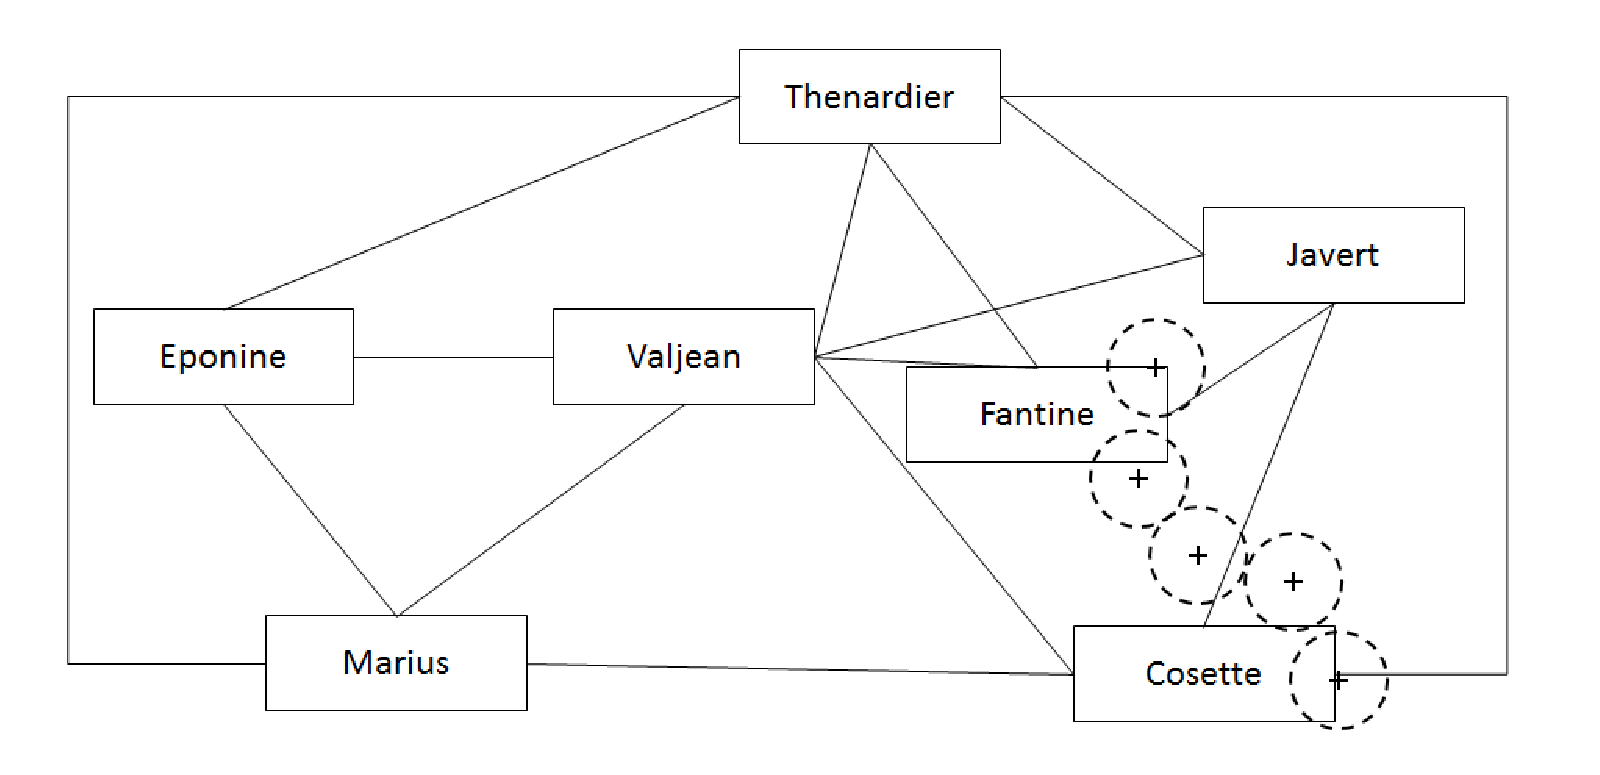
\includegraphics[width=0.99\linewidth]{images/MiserablesSimple.eps}
  \caption{: A network diagram with major characters of Les Miserables. The dashed circles represent a user's gazes. Here, most gazes are adjacent to Fantine and Cosette. }
	\label{fig:MiserablesSimple}
\end{figure}

Moreover, the visual objects shown in the Les Miserables visualization stand for actual data: the characters in the novel. So, mapping gazes to the visual objects lets us in turn map the user's interest to data elements, such as Fantine and Cosette. Moreover, by looking at the properties of the data that users are viewing, we can relate visual interest to semantic data subsets or perspectives. For example, Fantine and Cosette are both female characters and, based solely on the few gaze samples depicted in our example, we could conclude that the user is viewing female characters. In other words, we can track the user's interest in data subsets defined based on gender. Similar data subsets could be defined based on central or secondary characters, positive or negative characters, etc. We call this eye-tracking data analysis in ``data space'' or data of interest (DOI) analysis.

We hypothesize that this is a powerful alternative to traditional analysis methods, primarily AOI (area of interest) analyses. Using typical AOI-based approaches, analyzers would be required to define AOIs over already rendered 2D stimuli. In our example, and most real-life visualizations, this would be time-consuming because of the many visual objects shown on the screen. Moreover, the 2D layout of the visualization may change in response to user interactions (e.g., user moves node), in which case the AOI annotations would need to change. Moreover, AOIs are generally not annotated by any attributes so defining AOIs on characters wouldn't implicitly mean that we could also track other data subsets such as based on gender.  

However, as described in Chapter~\ref{chap:Intro}, mapping gazes to individual data objects is bound to be imprecise since eye-trackers produce noisy, low resolution data. Figure ~\ref{fig:MiserablesGaze} illustrates this. We can use the na\"{i}ve approach of mapping gazes to the nearest visual object. Using this approach, we can confidently map $g_1, g_2$ to Fontaine, and $g_4, g5$ to Cosette. However, it's less clear what we should do about $g_3$ since it's squarely between the two nodes. 

\begin{figure}[htb]
  \centering
  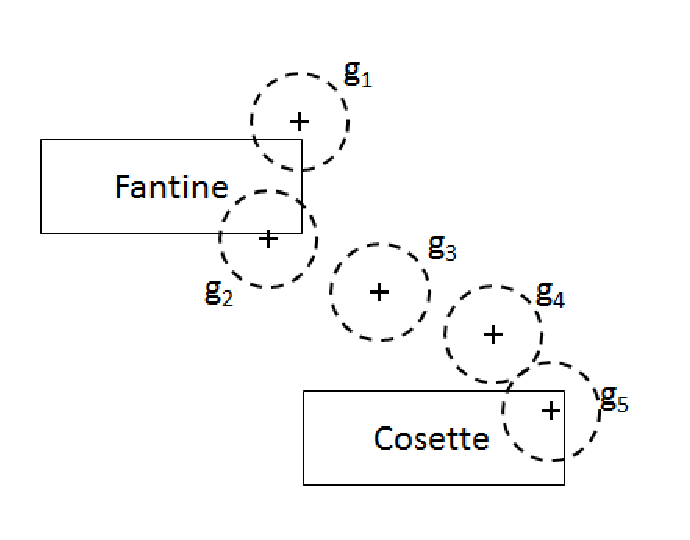
\includegraphics[width=0.5\linewidth]{images/MiserablesGaze.eps}
  \caption{: Using proximity alone to map gazes to visual objects. We have 2 rectangles Fontaine and Cosette, and five gazes $g_1, g_2, g_3, g_4, g_5$. Each gaze is to be mapped to either Fontaine or Cosette. $g_1, g_2$ maps to Fontaine and $g_4$ map to Cosette. However, $g_3$ cannot be mapped directly to neither Fontaine nor Cosette. }
	\label{fig:MiserablesGaze}
\end{figure}

As part of our proposed first contribution, we will attempt to create automatic methods that can map gazes to objects more accurately than using this na\"{i}ve approach. Tentative plans for such methods are described below in Section~\ref{sec:Algorithm}. We will test, and validate these methods, and the feasibility of the DOI approach to produce accurate data in general, by: (i) using the methods to instrument a concrete, representative visualization (described in Section~\ref{sec:TestCase}); (ii) gathering DOI data from human subjects using the visualization; and (iii) comparing the collected data to a ground-truth derived as discussed in Section~\ref{sec:Validation}. 


\subsection{Proposed Methodologies for Collecting DOI Data Accurately}
\label{sec:Algorithm}
Initially, we assume that our eye-tracking experiments will use visualizations which are accessible for instrumentation to programmers. Thus, graphical information (e.g. position, size, shape) of internal visualization primitives (e.g. circles representing nodes in a graph) are available at rendering time. 

Our proposed methods will only operate over visualizations with open source-code. This is a limitation of our work. However, we claim that open source code libraries are gaining popularity over proprietary applications. Figure~\ref{fig:WebUsageChart} shows a comparison between two popular visualization libraries: d3JS (open source-code) and FusionChart (proprietary application).

\begin{figure}[htb]
  \centering
  \includegraphics[width=0.99\linewidth]{images/WebUsageChart.eps}
  \caption{: Comparison of number websites using d3js and FusionChart in their homepages. Data collected from http://trends.builtwith.com/. }
	\label{fig:WebUsageChart}
\end{figure}

We aim to map gazes to visualization primitives using our viewed-object-detection algorithm. Our algorithm will seek to compute ``object viewing scores'' that express the likelihood that an object is viewed given a particular gaze sample. The viewed-object-detection algorithm outputs object viewing scores from which we can construct DOI data. We aim to develop viewed-object-detection algorithm incrementally in three stages. First, we plan to detect objects using the na�ve approach of AOI binning. We will consider each visual object as an AOI. In this method, the objects where most recent gazes landed will be considered as `viewed'. Second, we intent to develop a method for calculating a probabilistic fuzzy score for each object based on the proximity of gaze landing to the object. Third, we plan to build on Salvucci's method~\cite{Sal00} to develop an algorithm to calculate the object viewing score based on the probabilistic score and an additional prediction score. The prediction score will be calculated based on the semantic content in the data. 

\begin{figure}[htb]
  \centering
  \includegraphics[width=0.99\linewidth]{images/System.eps}
  \caption{: Detection of viewed objects in generative visualizations.}
	\label{fig:System}
\end{figure}

We depict our general approach for collecting DOI data in Figure~\ref{fig:System}. Eye-trackers supply gaze samples in screen space. The `Screen to Model Transformation' module (Figure~\ref{fig:System}) will transform these gaze samples to the visualization model space. The `Renderer' module will render the visualization, and supply information regarding shapes and positions of visual objects, and model transform information. Afterward, our algorithm will combine gaze samples and visual object positions to detect viewed objects by calculating object-viewing-scores. A prediction module will use information about what a user has viewed in the past and interacted with, to infer what objects the user is likely to be viewing presently. In Figure~\ref{fig:System}, we can see that gaze position and visualization information is passed to the viewed object detection module. We hypothesize that this will reduce the inaccuracies previously illustrated, by allowing us to discriminate which visual object is users is likely to be looking at, when gazes land near multiple objects.
More details about the three stages of developing viewed-object-detection algorithm are provided below. 

In our first stage, we will consider an objects is viewed if a gaze sample falls into it. This na\"{i}ve approach is impractical for a layout where objects are too large and too small, and with cluttering and overlapping. Thus, in our second stage, we aim to implement a probabilistic method for viewed object detection We will compute a fuzzy object gaze score $gs_{i,t}$ as  for each object $i$ in a visualization and at all times $t$ that range between zero and one. Gaze score value zero ($0.0$) interprets object i is not viewed. Moreover, gaze score value one ($1.0$) interprets object i is certainly viewed. 

Finally, in our third stage, we aim to extend the probabilistic method inspired from the contribution of Salvucci et al.~\cite{Sal00} to work for real-life visualization content. In Salvucci et al.'s method, an object iviewed  is calculated by solving Equation~\ref{eq:iViewed}. 

\begin{equation}
i_{viewed} = argmax_{i \in l}[Pr(g|i)\times Pr(i)]
\label{eq:iViewed}
\end{equation}

In Equation~\ref{eq:iViewed}, each object $i$ belongs to the list of all objects $l$. $Pr(g|i)$ is the probability of producing gaze position $g$, given $i$ is intended for viewing. Again, $Pr(i)$ is the prior probability of viewing $i$ at any time.  Similar to our probabilistic approach, we claim multiple visual objects in a visualization can be viewed rather than a single object. Thus, instead of detecting a single $i_{viewed}$, we calculate visual score $vs_{i,t}$  for each object $i$ and at all times $t$. The visual score is calculated using Equation~\ref{eq:vsit}. 


\begin{equation}
vs_{i,t} = gs_{i,t} \times ps_{i,t}
\label{eq:vsit}
\end{equation}

In Equation~\ref{eq:vsit}, $ps_{i,t}$ represents a prediction score for object $i$ at time $t$. Prediction scores are prior scores which generally depend on semantic content and visualization layout of visual objects. Moreover, analyzers may conduct pilot user studies and compute prior scores from the result data. Afterward, analyzers may use these prior scores as prediction scores in the next user study. We aim to achieve a similar method for computing prior scores.   


\subsection{Validation Methodology for Collected DOI Data.}
\label{sec:Validation}

Determining the accuracy of detecting viewed DOIs automatically is non-trivial because obtaining the ground-truth (i.e., what objects users actually looked at) is difficult. The main reason is that human perceive scene subconsciously and cannot reliably self-report what objects they have viewed. Moreover, different users may view the same object differently. Thus, we aim to obtain an approximation of the ground truth by asking human annotators to perform an offline, manual viewed object detection. In this process, we will ask the annotators to analyze recorded screen videos overlaid with gaze samples, and manually record which object the user might have viewed at each moment in time. Then, we will compare our automatically collected DOI data to analyzers' data in order to evaluate the similarity between them.  In effect, we will investigate if the automated method can provide results that are comparable in terms of accuracy with the state-of-the-art: a human coders' ability to infer from raw eye-tracking data what visual objects a user has looked at, only with less overhead and much faster.

The only other alternative would be to employ the `Think Aloud Protocol' (TAP) where users verbally say what they are looking at during their session. However, it is know that TAPs are unreliable because they distract users from their natural workflows. Also, information can be verbalized which can be actively processed in working memory~\cite{Jaa10}. Thus, TAP is unable to access full cognitive process. Moreover, TAP delays thought-process about 30 percent~\cite{Krings01}. User performance significantly differs comparing TAP and no TAP scenarios~\cite{Cooke05}. 

\subsection{Test case}
\label{sec:TestCase}

We will test the feasibility of DOI collection and evaluation into the context of a PivotPaths visualization~\cite{Dor12} generated from IMDB movie data. Figure~\ref{fig:PivotPath} shows an example of the PivotPaths visualization, in which actors, directors, and genres are connected to movies. The visualization is integrated with interactions such as zooming, panning, hovering, and clicking. As such, the visualization is ever-changing, making it extremely difficult to analyze using manual gaze data analysis techniques (e.g., AOI) and thus an appropriate test case that can capture the benefits of automatic DOI detection as compared to manual AOI workflows. Moreover, the visualization uses visual and interactive paradigms that are representative of real visualizations, and its underlying movie data is familiar to users participating in our validation studies. 

\begin{figure}[htb]
  \centering
  \includegraphics[width=0.99\linewidth]{images/PivotPath.eps}
  \caption{: PivotPaths visualization of IMDB data.Movies are displayed in the center of the screen, actors at the top, and directors and genres share the bottom space. Actors, directors, and genres associated to movies are connected through curves. Users can highlight objects and their connected neighbors by hovering over them.  }
	\label{fig:PivotPath}
\end{figure}


